%!TEX root=rapport.tex
	
\subsection{Alignement}
\label{subsection:alignment}
Les deux dernières étapes que sont l'alignement et le consensus sont 
implémentées dans la classe \verb|ConsensusAbstract| à travers les méthodes 
\verb|computeAlignment| qui calcule l'alignement des séquences et le sauvegarde 
dans l'attribut \verb|alignment| ainsi qu'à travers la méthode \verb|build| 
qui calcule le consensus.

Pour calculer l'alignement, nous utilisons les segments alignés ans l'ordre 
donné par l'algorithme greedy décrit à l'étape \ref{subsection:greedy}.
L'algorithme greedy nous ressort une liste de paires de séquences $P_{i}$ tel
que le deuxième segment de la paire $P_{i}$ provient du même segment initial que
le premier de la paire $P_{i + 1}$, la différence se situant dans les gaps
ajoutés lors de l'alignement semi-global entre les nucléotides pour offrir le
meilleur score pour chaque paire.

Pour pouvoir construire le contig final, il nous faut réaligner convenablement
chaque paire de segments et pour cela, nous allons propager les gaps qui ont été
ajoutés lors des calculs de l'alignement semi-global. Nous effectuons cette
propagation en deux temps:

\begin{enumerate}
	\item vers le bas, c'est-à-dire, pour une paire $P_{i}$ on regarde si, entre
		deux nucléotides de la deuxième composante de $P_{i}$, le
		nombre de gaps est plus grand qu'entre les deux mêmes nucléotides de la première
		séquence de la paire suivante $P_{i + 1}$ et si c'est le cas, on propage la
		différence entre ces nombres vers les séquences du dessous.
	\item vers le haut par le même procédé que pour la propagation vers le bas
		sauf que nous propageons les gaps qui sont plus présents dans la
		première composante de la paire $P_{i + 1}$ que dans la deuxième
		composante de paire $P_{i}$ et qu'on propage alors la différence de gaps
		vers les séquences du dessus.
\end{enumerate}

Grace à ce procédé, nous sommes sûrs que les séquences résultantes des
alignements semi-globaux sont bien les mêmes et que l'ordre renvoyé par le greedy
est toujours le même (car l'ordre des scores reste le même).

\subsubsection{Représentation d'une séquence pour l'alignement}

Au vu de cette méthode de propagation de gaps, le procédé d'alignement n'est
donc qu'un ajout de gaps entre nucléotides: il est alors intéressant de
représenter les séquences alignées comme des séquences sans gaps où, après
chaque nucléotide de la séquence, nous retenons, dans un tableau d'entier, le
nombre de gaps suivant celui-ci.\footnote{Une même représentation peut être
	utilisée pour représenter pour les nucléotides successifs identiques: nous
	compressons ainsi la séquence. Nous n'avons souhaité compresser que les gaps
	car nous n'allons travailler qu'avec ceux-ci, et cela aurait complexifié
l'implémentation des méthodes.}

Par exemple, la séquence \verb|A--T-G-C| sera représenté par une séquence
\verb|ATGC| et par un tableau nommé \verb|nb_gaps| de taille 4
contenant les entiers {2, 1, 1, 0} car il y a deux gaps après le premier
nucléotide, un gap après le second, un après le troisième, et 0 à la fin. Les
complexités en temps et en mémoire sont ainsi diminuées.
Au niveau de la mémoire, une séquence alignée se voit ainsi 'compressée'.

L'ajout de gaps sera alors très simple et très rapide en complexité. En effet,
si nous souhaitons ajouter un gap à la position 2 (supposons qu'on commence en
0) à la séquence \verb|A--T-G-C| pour obtenir \verb|A---T-G-C|, il nous suffira
d'augmenter de 1 le nombre de gaps après le nucléotide A: nous obtiendrons alors
le tableau {3, 1, 1, 0}. Cet ajout de gap peut se faire en $O(n)$ où $n$ est la
taille de la séquence \textit{initiale}. De plus, l'insertion de gaps ne demande
pas plus d'espace mémoire: qu'importe si nous devons insérer $2$ gaps ou $10000$
gaps.\footnote{Avec la représentation sous forme de byte (1 octet en Java),
	cette nouvelle abstraction est intéressante si nous devons ajouter plus de 7
	gaps entre chaque nucléotide (un entier prenant 8 octets), ce qui peut
arriver si nous travaillons sur de grandes séquences.}

Un autre point positif est qu'il est très facile de connaitre la position où nous
devons insérer des gaps s'il nous est demandé de rajouter $n$ gaps entre deux
nucléotides: il suffit de connaitre la position du nucléotide dans la chaine
initiale après lequel nous devons ajouter les $n$ gaps.

Cette abstractation des séquences est réalisée dans la classe
\verb|SequenceAbstract|.\footnote{Cela justifie le nom de la classe
	\verb|ConsensusAbstract| qui travaille avec des objets de la classe
\verb|SequenceAbstract|, et non \verb|Squence|.}

\subsection{Consensus}
\label{subsection:consensus}

Grace à l'alignement précédemment réalisé, nos paires $P_{i}$ et $P_{i + 1}$ ont
maintenant la même séquence respectivement en deuxième composante et en première
composante et toutes les séquences sont maintenant bien alignées. Pour
construire le contig final, nous allons parcourir chaque colonne de l'alignement
et prendre le nucléotide qui apparait le plus souvent. En cas d'égalité, nous
prenons par ordre alphabétique.


\begin{comment}
\subsection{Deuxième approche}

Dans cette section nous expliquons l'approche du calcul de la séquence finale exposé par Aline. 
L'idée est un peu différente, car au contraire de l'approche précédente, nous ne propageons pas physiquement les gaps mais travaillons sur les paires d'alignements en les parcourant de gauche à droite chacune à leur tour. Chaque paire d'alignement n'étant pas de la même longueur ni parfaitement alignés les uns en dessous des autres, il faut savoir se rappeler à quelle position de la séquence finale nous nous trouvons réellement lors du traitement. C'est ici que l'idée d'\emph{offset} intervient. Cette méthode nécessite un nouvel objet \verb|Counter| qui est un compteurr  permettant de retenir pour chaque colonne le nombre de $A$, de $C$, de $T$ et de $G$ qui ont été comptabilisés en une certaine position (pour un certain compteur) de la séquence finale. Une fois tous les compteurs récupérés pour toutes les positions de la séquence finale il suffit de récupérer le nucléotide ayant comptabilisé le maximum d'occurrences pour cette colonne.

Un premier test de l'implémentation de cette idée a été effectué sans tenir compte du fait que des gaps pouvaient apparaitre au sein même d'un alignement. Par exemple si on a l'alignement de $(f,g)$ puis celui de $(g,h)$, il se peut que les gaps internes au niveau de $g$ dans le premier alignement ne soient pas les mêmes que les gaps internes de $g$ au niveau du second alignement. 
Nous avons pour cela besoin d'un dictionnaire qui a un entier (une position possible dans la séquence finale) associe un compteur et de la notion d'offset. 

Pour mieux comprendre la notion d'offset, illustrons-la sur la situation de la figure~\ref{offset}. Lors du parcours de première paire d'alignement, l'offset est à 0 car $f$ est à gauche de $g$. On parcourt alors toutes les positions des deux alignements en créants de nouveaux compteurs car il n'en existe pas encore pour les positions couvertent par $f$ et $g$. 
Lorsqu'on va traiter l'alignement $(g,f)$ l'offset devient négatif car le nucléotide le plus à gauche à traiter est avant le nucléotide que l'on avait considérer comme étant en position 0 (le premier nucléotide de la séquence $f$). On parcourt alors cet alignement de la gauche vers la droite sachant que pour certaine position (celles déjà couvertent par l'alignement $(f,g)$) des compteurs existent déjà et qu'il nous suffit donc de les mettre à jour.
\begin{figure}	
		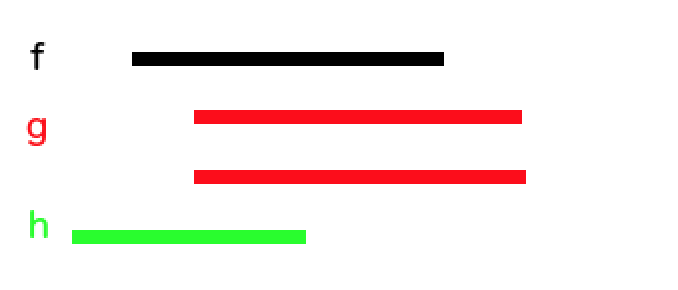
\includegraphics[scale= 0.50]{offset.png}
		\caption{Deux paires d'alignement $(f,g)$ et $(g,f)$}
		\label{fig:offset}
\end{figure}

Une telle approche, plutôt naïve, fournit déjà des résultats plutôt satisfaisants.
\end{comment}
